% File naaclhlt2010.tex
% Contact: nasmith@cs.cmu.edu
\documentclass[11pt]{article}
\usepackage{ijcnlp2011}
\usepackage{times}
\usepackage{url}
\usepackage{latexsym}
\usepackage{amsmath}
\usepackage{multirow}
\usepackage{url}
%\DeclareMathOperator*{\argmax}{arg\,max}
%\setlength\titlebox{6.5cm}    % Expanding the titlebox

\usepackage{arabtex}
\usepackage{amssymb}
\usepackage{caption}
\usepackage{epsfig}
\usepackage{subfigure}
\usepackage{color}
\usepackage{rotate}
\usepackage{rotating}
\usepackage{amsthm}
\usepackage{booktabs}

\usepackage{relsize}
\usepackage{fancyvrb}
\usepackage[colorlinks=false]{hyperref}

\usepackage{utf8}
\setarab
\fullvocalize
\transtrue
\arabtrue


%\newcommand{\CharCodeIn}[1]{`\CodeIn{#1}'}
\newcommand{\CodeIn}[1]{{\small\texttt{#1}}}
\newcommand{\frl}[1]{\fbox{\RL{#1}}} 
\newcommand{\noArRL}[1]{\arabfalse\RL{#1}\arabtrue} 
\newcommand{\noTrRL}[1]{\transfalse\RL{#1}\transtrue} 
\newcommand{\noTrnoVocRL}[1]{\transfalse\novocalize\noTrRL{#1}\vocalize\transtrue}  
\newcommand{\noVocRL}[1]{\transtrue\novocalize\RL{#1}\vocalize}  

%\title{Instructions for NAACL HLT 2010 Proceedings\Thanks{This...}}
\title{Automatic Hadith Graphs using Arabic Morphological Analysis}

%\author{ Jad Makhlouta \\\And
%Hamza Harkous \\
%  American University of Beirut \\
%  {\tt \{jem04, hhh20, fz11\}@aub.edu.lb } \\\And 
%  Fadi Zaraket 
%}

\date{}

\begin{document}

\maketitle

\begin{abstract}
\end{list}
A hadith in Islamic literature is a narration from the 
prophet Mohammad related by multiple narrators.
Establishing the authenticity of a hadith is an important task
based on which Islamic scholars issue rules that affect the life
of people around the world. 
The literature lacks an automated and exhaustive mechanism of 
authentication checks. 
This is currently manual work prone to error and almost
impossible to complete in the life time of a scholar due to the
large literature available. 
In this paper, we present a tool that uses 
an Arabic morphological analyzer 
to successfully automate the
analysis of three books of hadith selected 
arbitrarily and abstract 
each book into a graph of narrators related to each other. 
\end{abstract}

\section{Introduction}

A \RL{.hady_t}~\footnote{In this document, 
we use the default ArabTeX transliteration style ZDMG.}
(tradition) 
is a narration related to the prophet Mohammad
through a \RL{sanad} or a sequence of narrators. 
The collections of traditions are the second source of
jurisprudence after the \RL{qor'An} for all Islamic schools of thought. 
Figure~\ref{f:exhadith} shows an example \noArRL{.hady_t} in 
Arabic with its transliteration and translation. 
We show proper names in boxes connected
to form complex names of narrators. 
For example, 
\novocalize
\noTrRL{qtybT} is the first name 
of narrator $n_1$, and 
\noTrRL{s`yd} is the name of his father as 
the word \noTrRL{bn} (son of) indicates. 
The sequence of names from $n_1$ to $n_5$ 
constitutes the \noArRL{sanad} 
of the \noArRL{.hady_t}. 
The second part of the \noArRL{.hady_t} is the 
\RL{matn} (content) and constitutes the actual content 
of the tradition.

Due to religious and political reasons, 
writing the traditions was forbidden 
until the days of the eighth Umayad Calif,
\novocalize
\RL{`mr bn `bd al`zyz}(717-720 AC), seventy or so years after 
the death of the prophet~\cite{AlAskari}. 
Consequently, many inconsistencies were
introduced to the literature which necessitated 
a thorough authentication study of a tradition before its use in 
jurisprudence.
\vocalize
%An Islamic hadith scholar studies the authenticity of 
%the \noArRL{sanad} of a 
%set of related traditions before using these traditions 
%jurisprudence. 
While different Islamic schools of thought differ on 
how to interpret the content, they almost all agree
that if a \noArRL{sanad} lacks authenticity, 
then scholars can not use the tradition for jurisprudence.

The authenticity of a \noArRL{.hady_t} depends on 
the credibility of the narrators as reported in 
separate biography books. 
The study of \noArRL{.hady_t} authentication is 
currently manual and error prone due to the huge number
of existing traditions and tradition books. 
Hadithopedia~\cite{Hadithopaedia:08}
reports that the tradition and biography
books for one of the Islamic sects amounts to more than 
300 thousand lines of text. 
Al-Azami\shortcite{Al-Azami-91} cites more than eleven books
of digitized tradition books each of several volumes, and a dozen
other biography and secondary authentication books such
as a geographical dictionary of places in hadith. 

\novocalize

\transfalse
\begin{figure}[tb]
\center{
\resizebox{.9\columnwidth}{!}
{ \input{figs/exhadith.pdftex_t}}
\caption{Hadith abstraction example.}
\label{f:exhadith}
}
\end{figure}
% the FSMs for the three words
\transtrue
\vocalize

In this paper, we present the hadith {\em narrator graph
extractor using morphological analysis} (NaGEMA), 
a novel technique that automates
extracting the \noArRL{sanad} from the books of traditions 
into a diagram of chains of narrators. NaGEMA segments
a book into narrations, each narration into its \noArRL{matn} 
and its \noArRL{sanad}, 
and each sanad into its separate narrators. 
This work will lead to 
automate an exhaustive \noArRL{.hady_t} authentication 
effort in the future as we plan to 
automatically analyze the biography books.


%Automated analysis of Arabic data sets, including texts, 
%publications, records and digital media is essential
%with the huge digital Arabic content available nowadays. 
\subsection{ Arabic morphological analysis}
Arabic morphological analysis is key to our analysis. 
Current morphological analyzers~\cite{Sughaiyer:04}
use concatenative analysis when
considering the internal structure 
of an Arabic word and
composing it into several {\em morphemes}. 
A morpheme can be a {\em stem}, or an {\em affix}.
An affix can be a {\em prefix, suffix, } or an {\em infix}.
%The analysis of one word may lead to several possible
%morphological solutions.
\vocalize
The word \RL{'a.hmadH}
may have two valid morphological analyses. 
The letter \RL{'a} may be a prefix and the word means 
``I praise him'', or 
%The letter \RL{'a} may also be 
part of the stem \RL{'a.hmad} (a proper noun)
and the word means ``his Ahmad''.

The morphological analysis of the word \RL{.hd_tnA} 
``narrated to us'' that starts the hadith in Figure~\ref{f:exhadith}
returns the stem \RL{.hd_t}.
The stem  \RL{.hd_t} is also the stem of other 
words such as \RL{.hd_tny} and \RL{.hd_thm}.
The stem also shares similar part of speech (POS)
and English meaning gloss annotations with words
such as \RL{qaal} ``said'' and \RL{'a_hbar} ``told''. 
The use of morphological analysis allows us to 
subsume listing these stems and all of their morphological
derivations with one rule that matches the gloss and 
POS tags. 
Similarly the words \RL{ibn} ``the son of'' and \RL{bn} 
return the same morphological analysis.
         


\novocalize
%The accuracy of the solutions suffer due to inherent difficulties
%of morphological analysis of the Arabic language. 
%For example, it is common practice to write Arabic text
%without short vowels. 
%This greatly increases the ambiguity of Arabic text. 
%Arabic letters can have up to 
%four different forms
%corresponding to their position in a word, i.e, beginning,
%middle, end of word and separate forms. 
%This allows the phrase \transfalse
%\RL{il_A\nospace almdrsT} \transtrue
%to be visually recognizable
%as two separate words \RL{il_A} (to) and \RL{almdrsT} (the school) 
%without the need of a space in between. 
%The reason is the first word \RL{il_A} ends with
%\RL{_A} a non-connecting letter. 
%These words,
%referred to as ``run-on'' words~\cite{Buckwalter:04},
%occur often, and greatly increase the
%difficulty of tokenization.

Current morphological analyzers such as 
Buckwalter~\shortcite{Buckwalter:02},
Beesley~\shortcite{Beesley:01},
SAMA~\cite{Kulick:10},
and ElixirFM~\cite{Otakar:07} 
take as input white space delimited tokens~\cite{Kulick:10},
consider them as words,
and enumerate all possible solutions. 
This approach has several problems. 
First, a white space delimited token may have 
more than one word, referred to as ``run-on'' 
words~\cite{Buckwalter:04}.
Second, the exhaustive enumeration may not be efficient and may
not be necessary or appropriate
in some applications as noted in~\cite{Maamouri:10}. 
%Other morphological analyzers such as 
%Amira~\cite{Diab:07,Benajiba:07},
%MAGEAD~\cite{Habash:05}, and MADA+TOKAN~\cite{Habash:09} 
%use machine learning and support vector machines (SVM) 
%to disambiguate the morphological analysis at the expense 
%of efficiency. 
%Xerox rules can be compiled into specialized finite state
%machine (FSM) based analyzers as described in~\cite{Beesley:03}.
%However, the efficiency of the resulting analyzer depends on the
%way the Xerox rules are written. 
%This requires deep knowledge and insight from the user
%in compilation techniques, context free grammars, 
%and morphological analysis.
%context free grammar rules that can be automatically compiled
%into efficient non-deterministic finite state Automata (NDFSA). 

%\subsection{Sarf}
%\label{sec:intro:sarf}

{\bf Sarf.~~~}
Sarf~\footnote{Sarf (name modified for blind review) }
is 
an {\em application-specific efficient
morphological analyzer} based on
non-deterministic finite state Automata 
driven by an application-specific controller customized 
by the user. 
%Each machine in Sarf takes one letter at a time as input
%and represents a valid morphological analysis.
The application-specific controller prunes false positives
early in the run by making a decision at every input letter
to control the machines.
Sarf builds on and extends the lexicon of 
Buckwalter~\shortcite{Buckwalter:02} 
with proper and location names extracted from different online 
sources~\footnote{\href{http://alasmaa.net/}{http://alasmaa.net/ }, 
\href{http://ar.wikipedia.org/}{http://ar.wikipedia.org/}}
%as well as biblical sources~\footnote{Genesis 4:17-23; 5:1-32; 9:28-10:32; 11:10-32; 25:1-4, 12-18; 36:1-37:2; Exodus 6:14-25; Ruth 4:18-22; 1 Samuel 14:49-51; 1 Chronicles 1:1-9:44; 14:3-7; 24:1; 25:1-27:22; Nehemiah 12:8-26; Matthew 1:1-16; Luke 3:23-38}.
as well as biblical sources.
%~\footnote{Genesis 4:17-23; 5:1-32; 9:28-10:32; 11:10-32; 25:1-4, 12-18; 36:1-37:2; Exodus 6:14-25; Ruth 4:18-22; 1 Samuel 14:49-51; 1 Chronicles 1:1-9:44; 14:3-7; 24:1; 25:1-27:22; Nehemiah 12:8-26; Matthew 1:1-16; Luke 3:23-38}.

%Each alive machine in Sarf takes as input one letter at a time 
%from a text stream. 
Sarf does not assume that the word at hand is a token and
performs tokenization on the fly based on morphological correctness
and thus can handle 
the ``run-on'' words problem. 
Sarf also uses diacritics if they exist to disambiguate 
morphological solutions. 

In this paper we make the following contributions. 
\begin{itemize}
\item We automate the segmentation of hadith books into separate narrations and extract chains of narrators into a partial order relation graph using a knowledge based approach with morphological analysis.
\item We introduce a specialized distance metric for Arabic names used in Arabic literature. 
\item We provide a working and efficient implementation of
our work. 
\end{itemize}

The rest of this paper is organized as follows. 
We describe our approach to narrator chain extraction
in Section~\ref{sec:islamic}.
We describe how we build the partial order relation
graph in Section~\ref{sec:graph}.
We discuss related work in Section~\ref{sec:related}.
We present our results in Section~\ref{sec:results} and 
we conclude in Section~\ref{sec:future}.

%The hadith 
%application specific controller that controls Sarf considers 
%proper names and ignores text where
%proper names occur rarely.
%It also considers words that relate names to each other 
%such as \RL{bin} or ``the son of''
%and words that mean narrate such as \RL{qaal} or ``said''. 

%With Sarf, we successfully automated the analysis of 
%three books of Islamic narrations~\cite{IbnHanbal,AlTousi,AlKulayni}
%and extracted from each one of them a vector of complex structures 
%that are three level deep in hierarchy.
%We also merged these vectors into a graph of narrators where 
%we represented identical narrators from separate traditions 
%in one single node. 

%The rest of this paper is structured as follows. 
%In Section~\ref{sec:sarf}
%we discuss Sarf and illustrate it with a running example.
%We also explain how non-deterministic finite state Automata
%work. 
%In Section~\ref{sec:islamic} we present the hadith application. 
%We present our results in Section~\ref{sec:results}.
%In Section~\ref{sec:related}
%we compare NaGEMA to related work. 
%We conclude with future work in Section~\ref{sec:future}.

%\section{Background}
% TODO: nondeterministic finite-state automata



%The survey in~\cite{Sughaiyer:04} compares
%several morphological analyzers. 
%Analyzers such as~\cite{Khoja:01,Darwish:02} 
%target specific applications in the 
%analyzer itself or use a specific set of POS tags
%as their reference.
%Sarf differs in that it is a general morphological 
%analyzer that reports all possible solutions. 
%It is case-based in the sense that a controller 
%prunes these solutions. 
%
%Sarf builds upon the lexicon of Buckwalter\shortcite{Buckwalter:02}.
%It differs from Buckwalter in that it defines a shorter list of affixes
%and a longer list of affix compatibility rules to allow 
%affixes to be defined recursively
%so that we can have prefix-prefix an suffix-suffix 
%concatenations.
%This allows Sarf to better maintain and propagate 
%the POS tags associated with affixes. 
%%This information is highly 
%%redundant with Buckwalter.% and that may lead to consistency issues. 
%Sarf keeps all the possible analyses alive where each analysis
%corresponds to a set of decisions and positions in the text. 
%Buckwalter produces a set of solutions for each token 
%and the several analysis threads of the text need to be 
%generated as a product of the token solutions. 
%
%Similar to Sarf, Beesley~\shortcite{Beesley:01} uses
%finite state Automata (FSA). 
%It reports that the number of Automata generated by a compiler
%for Xerox rules can not be controlled and also reports a difficulty 
%to compose the FSAs into a single framework. 
%Sarf however constructs an NDFSA from
%the controller and the prefix, stem, and suffix deterministic 
%transducers to solve the problem.
%Sarf also differs in that it uses recursive affixes in the 
%affix transducers, and in that the transducers consider
%input from the controller to modify their behavior. 
%%With Sarf it is easy to control the FSA with a case-based
%%controller. 
%Beesley requires recompilation of the Xerox rules.
%
%Similar to The MADA+TOKAN toolkit, Sarf thinks of
%the several valid morphological analyses as a richness that 
%should be exploited at a higher abstract level rather than
%an inaccuracy that should be corrected. 
%Sarf differs in that it provides an interface for the 
%case study to interfere in judging the analyses much earlier and
%at a finer granularity level. 
%In Sarf, there is no need for a separate tokenizer such as
%TOKAN since each solution keeps a stack of positions
%that partition text into morphemes.
%%The case-based controller can build the trace 
%%when needed. 
%
%%MAGEAD 
%%Maamouri, Mohamed and \bgroup et al.\egroup },
%
%Our approach is close to the refinement of SAMA~\cite{Maamouri:10}.
%SAMA was refined to interact with
%the ATB~\cite{Maamouri:04} project after the addition of a large 
%new corpus. 
%%We find supporting evidence in this decision to our hypothesis
%%about the utility of a case-based analyzer. 
%The algorithmic changes in SAMA were
%done manually and worked in integration with the ATB format. 
%Sarf is a case-based controller approach that can modify 
%the behavior of the analyzer on the fly and can interact
%with any case study. 
%%In Sarf, the analyzer remains general, and the 
%%case-based controller specializes the analysis.
%
%The AMIRA~\cite{Diab:07} analyzer uses 
%a language independent SVM based analysis. 
%The SVM analysis learns features from the input text 
%and does not make use of any information 
%in the target query.
%
%Like ElixirFM~\cite{Otakar:07}, Sarf builds on the lexicon
%of the Buckwalter analyzer. 
%Sarf also uses deterministic parsing with tries 
%to implement the affix and stem transducers. 
%We think that the inferential-realizational approach 
%of ElixirFM
%that is highly compatible with the Arabic linguistic 
%description~\cite{Badawi:04}
%can benefit from many features unique to the Arabic language.
%Sarf leaves implementing that to the case-based controller
%since in many cases the abstraction needs only a partial 
%linguistic model of the Arabic language. 
%%We can compare the case-based controller in Sarf to a high level
%%component in the ElixirFM domain specific language. 
%

%Sarf encodes the prefix, suffix and stem lexicons into
%three deterministic transducers and 
%uses a non-deterministic construction
%of the three to compute all valid morphological analyses.
%We first present a running example of Sarf.
%The running example explains how Sarf works,
%implements recursive affixes, and
%handles ``run-on'' words.
%Then we discuss how Sarf builds and composes the different FSAs.

\section{Narrator chain extraction }
\label{sec:islamic}

\begin{figure*}
\center{
\resizebox{1.9\columnwidth}{!}
{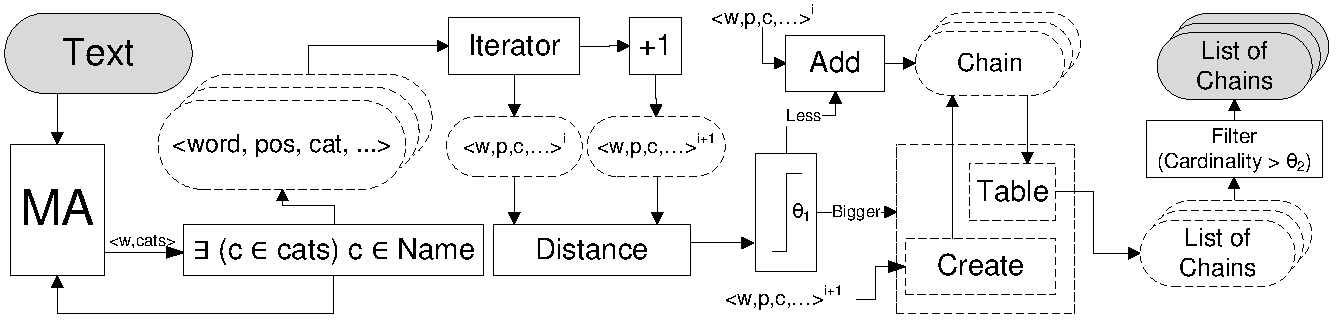
\includegraphics{figs/detailed_submachine.pdf}
}
\caption{The chain of narrators extractor diagram}
\label{f:chain}
}
\end{figure*}

%Several researchers~\cite{Hadithopaedia:08} attempted to automate 
%the analysis of the hadith literature. 
NaGEMA uses Sarf to automate the
analysis of three books of hadith selected 
arbitrarily~\cite{IbnHanbal,AlKulayni,AlTousi}\footnote{We obtained
  the digitized books from online sources such as 
  \href{http://www.yasoob.com/}{http://www.yasoob.com/} and 
  \href{http://www.al-eman.com/}{http://www.al-eman.com/}. }.
%  Our understanding is that those books are historical documents with 
 % public IP.}.
%\setcode{utf8}
%\begin{arabtext}
%حدثنا \emphasize{هشيم}، أخبرنا \emphasize{إسماعيل بن أبي خالد}،
% عن أبي إسحاق، عن سعيد بن جبير، قال كنا
%    مع ابن عمر رضي الله عنه حيث أفاض من
%    عرفات إلى جمع فصلى بنا المغرب ومضى
%\end{arabtext}
%\setcode{standard}
NaGEMA accepts a book as input
and segments it into a vector of hadiths. 
NaGEMA segments each hadith into its
sanad and matn parts. 
NaGEMA 
detects the chain of narrators in the sanad and 
the relation that links each narrator to his ancestor and 
predecessor in the chain. 
It also detects the full name of each narrator that is
composed of several proper names with connectors
in between. 

To do that NaGEMA queries Sarf for the following morphological 
categories.
\begin{itemize}
\item $\mathit{NAME}$: a proper name of a person such as \RL{'a.hmad} .
\item $\mathit{IBN}$: a special name connector meaning the son of such as \RL{ibn}.
\item $\mathit{NMC}$: other name connectors that may be any word appearing amongst the other interesting categories. 
\item $\mathit{NISBA}$: a possessive adjective that qualifies a person such 
as \RL{alma.sriy} ``the Egyptian''. 
\item $\mathit{NRC}$: a narrator connector such as
\RL{`an} ``on behalf of'', \RL{.hada_t} ``narrated'', \RL{qaal} ``said'', 
\RL{'a_hbar} ``told'' or one of their morphological equivalents. 
\end{itemize}


The diagram in Figure~\ref{f:chain} describes 
the chain extraction process. 
We pass the hadith to the morphological analyzer 
and check the returned words and category pairs 
for name categories.
Next we compute the number of words between every two names
and compare that to a threshold $\theta_1$.
If the name is within the threshold we add it to a temporary 
chain of names. 
Otherwise, we 
{\bf 1.} tabulate the chain into a temporary table containing 
the list of chains and
{\bf 2.} Create a new chain with the last element.
Finally, we filter out those chains whose cardinality 
is less than some threshold  $\theta_2$.

The process also benefits from name connector 
words and narrator connector words to enhance the
accuracy of the chain extraction and to segment the 
chain accurately into narrators.
Once we meet a name connector or a narrator 
connector word we reset the word counters that we
compare against the thresholds. 



\subsection{The hadith controller}
\label{sec:controller}
% FSM for the controller

We implemented our hadith chain extraction 
in a finite state machine
controller that interfaces with Sarf.
Intuitively, the controller reports a valid chain 
of narrators when a sequence of names
connected by narrator connectors appears. 
%This includes the task of finding multi-word names
%such as \RL{`bd alr.hmn} often appearing as ``run-on'' words.
The controller marks the beginning of the hadith with 
the beginning of 
the current proper name sequence,
and marks the end of the hadith with the beginning of the 
next proper name sequence. 
It detects the chain of narrators as the sequence itself. 

%The controller also targets words that mean ``narrate'' when
%they appear between proper names. 
We illustrate the hadith controller 
in Figure~\ref{f:hadith}. 
The transitions are labeled using expressions
that operate on the output tags 
generated from the Sarf morphological analyzer.

The controller has four states that correspond to 
a position in text relative to the next sanad. 
State $\mathit{TEXT\_S}$ is the initial state and denotes 
that the controller is outside the context of a sanad.
State $\mathit{NAME\_S}$ denotes that the controller is in
the middle of a chain and has last met a name. 
State $\mathit{NMC\_S}$ denotes that the controller is in
the middle of a narrator name.
State $\mathit{NRC\_S}$ denotes that the controller is 
in the context of a narrator name and the controller 
has met a narrator connector and is ready to meet 
a new narrator. 

The threshold $\theta_{\mathit{nmc}}$ 
corresponds to the number of tolerated name connectors 
that may occur between two names. %3
The symbol $\mathit{LIST}_{\mathit{nmc}}$ corresponds to the list 
of name connectors collected since the controller
started looping in the state $\mathit{NMC\_S}$.
The symbol $\lambda_{\mathit{nmc}}$ is a parameter 
that corresponds to a relaxed tolerance measure that
the controller resorts to in case the words separating
two names were longer than $\theta_{\mathit{nmc}}$ but 
contained a name connector word such as $\mathit{IBN}$ 
or $\mathit{NISBA}$.

The controller moves to state $\mathit{NAME\_S}$ on
$\mathit{NAME}$.
It moves to state $\mathit{NRC\_S}$ 
when Sarf reports an $\mathit{NRC}$.
State $\mathit{NMC\_S}$
indicates that the controller expects a name to appear within 
a tolerance threshold expressed by 
$\theta_{\mathit{nmc}}$ and $\lambda_{\mathit{bmc}}$.
It returns to $\mathit{NAME\_S}$ when a name is met, 
loops when still within the threshold, and 
resets to $\mathit{TEXT\_S}$ when the threshold is exceeded 
signaling that the last collection of names met do not qualify
as a narrator or a chain of narrators. 

Similarly, $\mathit{NRC\_S}$ tolerates $\theta_{\mathit{nrc}}$ words 
before it gives up on its expectations. 
Note that we reach the $\mathit{NAME\_S}$
state only when a
valid $\mathit{NAME}$ is detected and we leave when no 
more $\mathit{NAME}$'s are detected.
The $\mathit{NRC\_S}$ state can only be reached if an 
$\mathit{NRC}$ is detected.
The state $\mathit{NMC\_S}$ can only be reached from a 
$\mathit{NAME\_S}$ state.
We used the values of 3, 5 and 5 for $\theta_{\mathit{nmc}}$, 
$\lambda_{\mathit{nmc}}$, and 
$\theta_{\mathit{nrc}}$ respectively to run the experiments 
we report in Section~\ref{sec:results}.

\begin{figure}[tb!]
\center{
\resizebox{.9\columnwidth}{!}
{ \input{figs/hadith.pdftex_t}}
\caption{The controller of the hadith application.}
\label{f:hadith}
}
\end{figure}

%The definition of input labels such as NAME and IBN depends on the 
%morphological analyzer. 
%However, our case-based controller approach was able to perform well
%under both Sarf and a refined version of Sarf.

\subsection{Optimizations}

In addition to the controller, 
NaGEMA uses punctuation marks to refine its analysis and 
increase the accuracy of name detection, narration detection and narrator boundaries. 
It also learns narrator names from simple patterns that 
happen within narrator connectors and that are not 
reported by Sarf as names. 
NaGEMA learns names of narrators that consist of words missing from 
the Sarf lexicon.
NaGEMA learns the narrator names based on their context as they occurred 
between narrator connectors or contained name connectors. 

\section{The narrator graph}
\label{sec:graph}

\begin{figure}[tb]
\center{
\resizebox{1.1\columnwidth}{!}
%{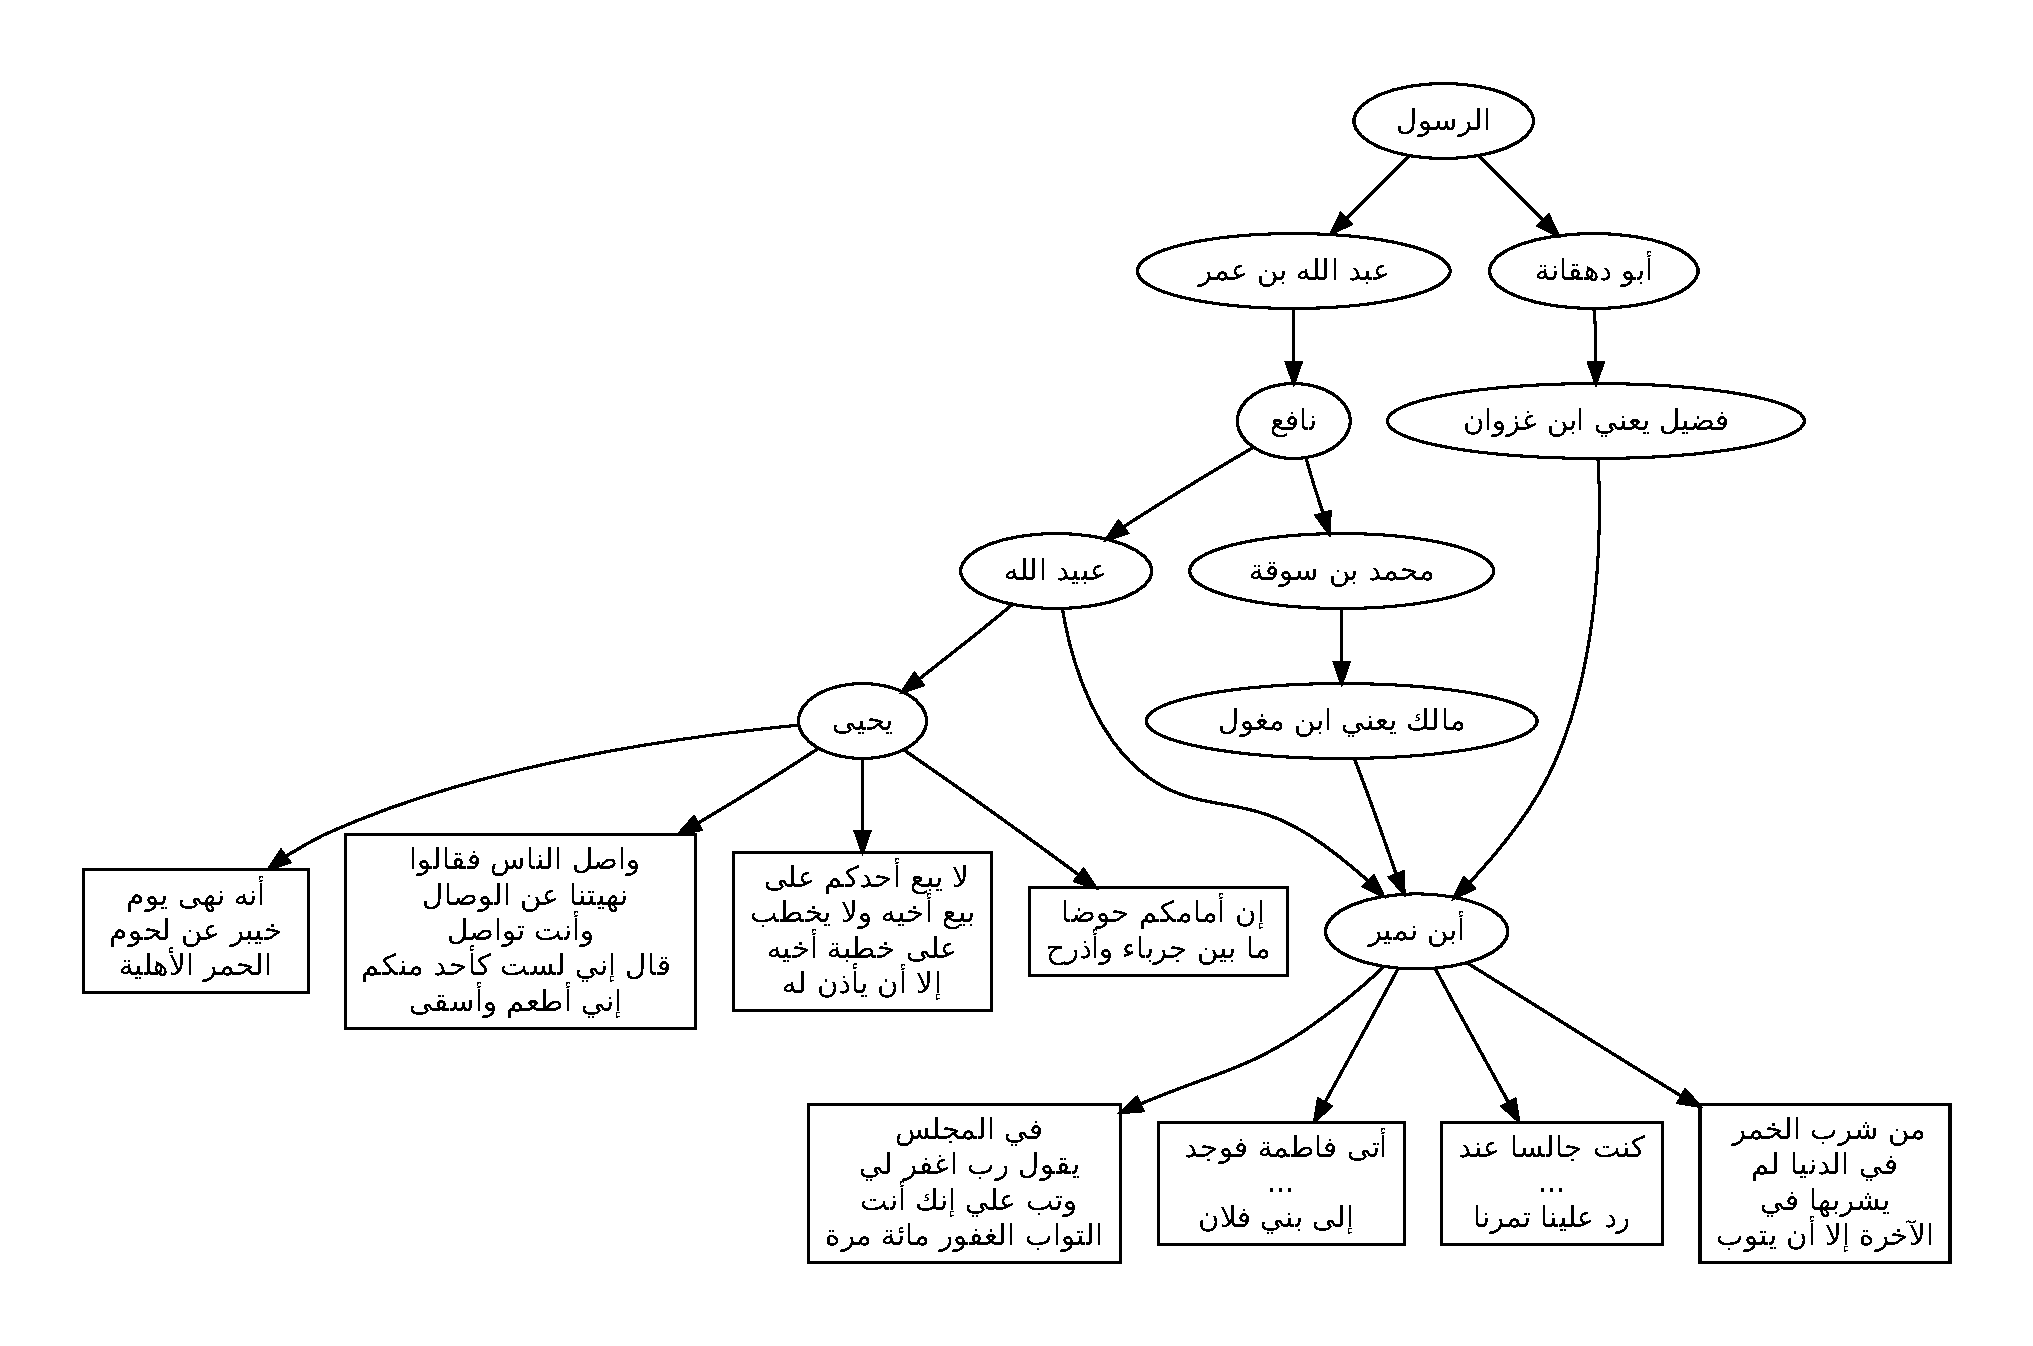
\includegraphics{figs/narrator_chain_output.pdf}}
{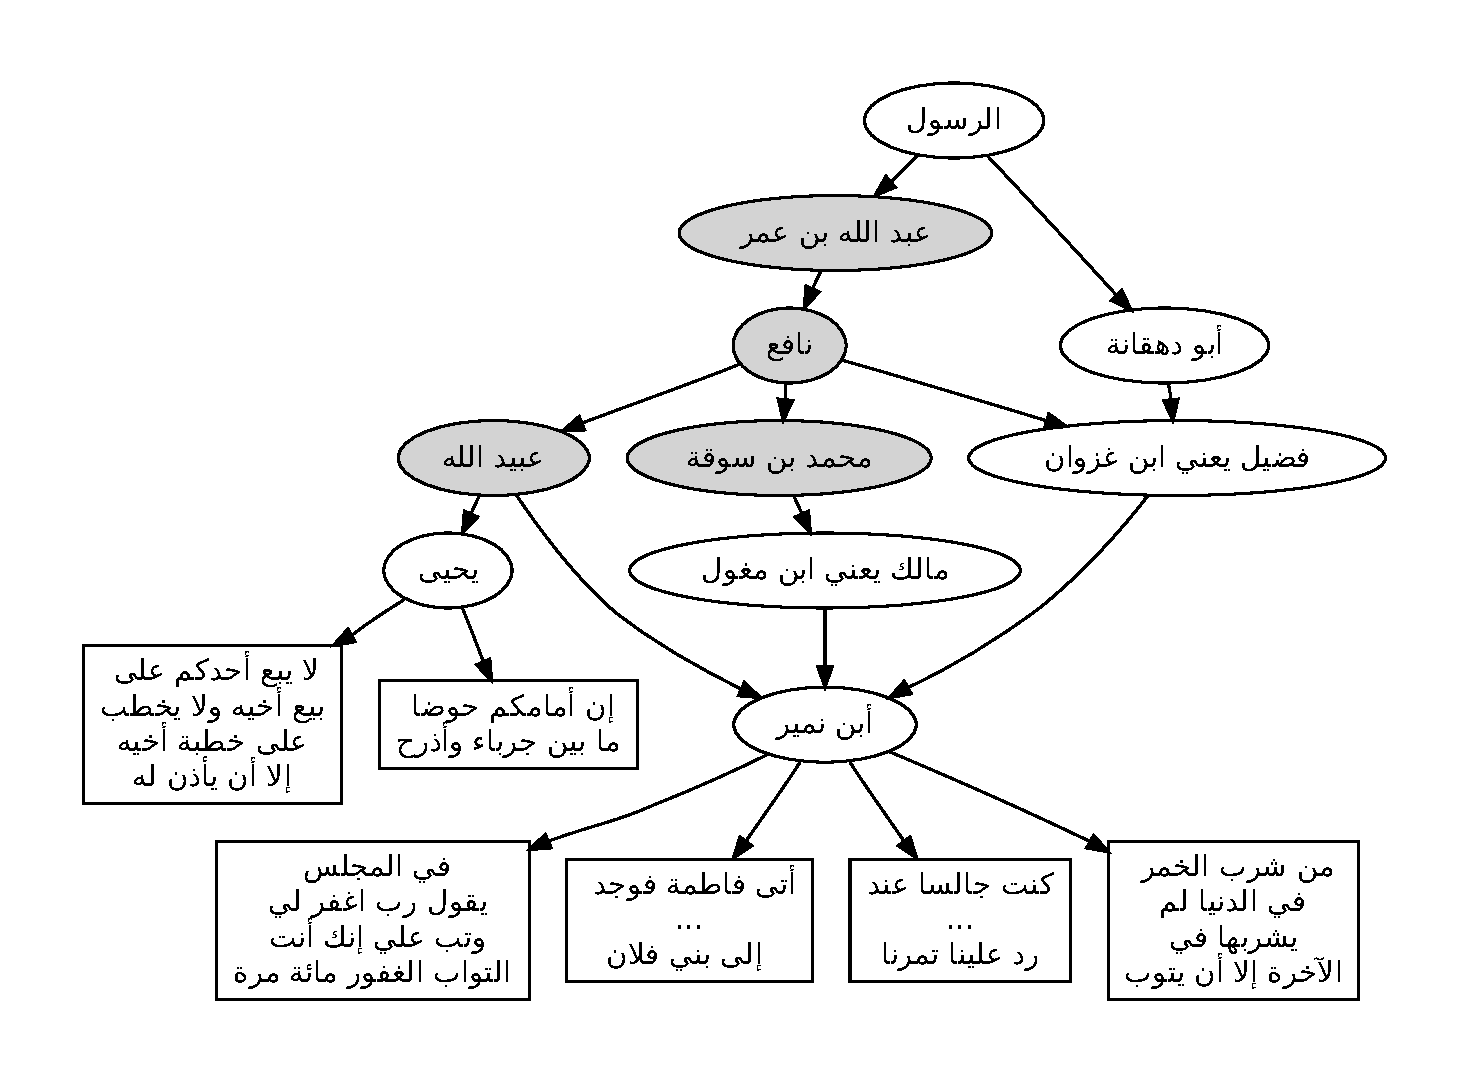
\includegraphics{figs/DAG_narrator.pdf}}
\caption{Narrator directed acyclic graph 
    extracted using NaGEMA }
\label{f:narrators} 
}
\end{figure}

The directed acyclic graph (DAG) 
in Figure~\ref{f:narrators} shows a partial order 
relation (POR) between narrators.
We automatically extracted the POR from the three books of 
hadith~\cite{IbnHanbal,AlKulayni,AlTousi}.
The nodes in boxes are the \RL{matn} of the hadith, 
and the other nodes are the narrators.
Given a set of chains of narrators similar to 
Figure~\ref{f:exhadith} we formed the DAG using graph algorithms 
that merged equal names in the chains. 

\subsection{Motivation}

The hadith POR is instrumental to automate
localization of narrators in biography documents and
to segment biography documents in future work.
Consider a biography that discusses a narrator.
It mentions his professors and students.
We plan to segment the biographies with a graph 
coloring algorithm
that parses the text looking for names. 
Once a name is found it locates it in the POR graph
and colors the POR node corresponding
to it.
The narrator predecessors in the POR are supposed to be
his professors and the narrator successors in the POR 
are supposed to be his students. 
Consequently, whenever a name moves away from the 
colored local cluster in the POR graph, 
we know that we are within a new biography. 

Once the biographies are analyzed, we can annotate
the POR with qualifiers of the narrators that reflect
their authenticity. 
We can also annotate the POR with the locations and 
the time the narrators lived in. 
Then we can check for time and location overlap
to discover inconsistent narrations.
This motivates our interest to automatically generate 
the POR graph.


\subsection{Graph merge Algorithm}

(modify according to hash)

\begin{table}[tb]
%\centering
%\resizebox{.9\columnwidth}{!}{
\begin{tabular} {p{6cm}}
\begin{Verbatim}[fontsize=\relsize{-2},
frame=topline,framesep=4mm,label=\fbox{Merge Algorithm},
commandchars=\\\{\}, codes={\catcode`$=3\catcode`_=8}]
Merge(Chain $C$[])
  Chain $C_c$[]=\{\}
  foreach Chain $c_1$ in $C$ 
    $C_c = C_c \cup c_1$
    foreach Chain $c_2$ in $C-C_c$
      foreach Narrator $n_1$ in $c_1$
        start = max( $n_1$.index - radius, 0)
        end = min($n_1$.index + radius, $n_2$.size)
        $n_2$ = $c_2$[start]
        while (true)
          if (Distance($n_1$, $n_2$) < $\theta$)
            mergeNodes($n_1$, $n_2$)
          if ($n_2$ = $c_2$[end])
            break
          $n_2$ = $c_2$.next($n_2$)        
\end{Verbatim}
\end{tabular}
%}
\label{t:merge}
\end{table}


The \CodeIn{Merge} Algorithm 
iterates over the chains of narrators looking 
for equivalent narrators and merges the equivalent
narrators.
The \CodeIn{radius} parameter refines the search 
to only consider narrators who belong to the same 
generation. 
For example, a narrator relating directly to the prophet
is definitely not equivalent to a narrator separated
from the prophet by ten or more narrators. 



\begin{table}[tb]
%\centering
%\resizebox{.9\columnwidth}{!}{
\begin{tabular} {p{6cm}}
\begin{Verbatim}[fontsize=\relsize{-2},
frame=topline,framesep=4mm,label=\fbox{Narrator distance metric },
commandchars=\\\{\}, codes={\catcode`$=3\catcode`_=8}]
Distance(Narrator n1, Narrator n2)
  $N_1$ = stems(n1.names)
  $N_2$ = stems(n2.names)

  $E_n$ = getEqualNames($N_1$, $N_2$)
  if ( $E_n$.isEmpty ) 
      return $\infty$
  if ( $E_n$.size $\ge$ min($N_1$.size,$N_2$.size))
    dist -= $\delta_1$
  if ($E_n$.equalNamesInOrder())  
    dist -= $\delta_2$

  $I_1$ = extractIbn( stems(n1.connectors) )
  $I_2$ = extractIbn( stems(n2.connectors) )
  $C_1$ = stems(n1.connectors - $I_1$)
  $C_2$ = stems(n2.connectors - $I_2$)
  if ($C_1 \cap$ Places $\not= C_2 \cap$ Places)
    dist += $\delta_3$
  else
    dist -= $\delta_3$

  $E_c$ = getEqualConnectors($C_1$, $C_2$)
  dist -= $E_c$.size * $\delta_4$ 

  if (correctIbnCorrespondence($I_1$, $I_2$))
      dist -= $\delta_5$
  return (MAX - dist)
\end{Verbatim}
\end{tabular}
%}
\end{table}

\subsection{Narrator morphological distance metric}

The \CodeIn{Distance} Algorithm 
takes as input two narrators and returns 
their morphological and order distance
from each other. 
The lower the distance is, the more
equivalent the narrators are. 

Each narrator has several names and several name and 
narrator connectors. 
\CodeIn{Distance} computes the names of the two narrators
and stores them in $N_1$ and $N_2$ 
and checks whether they are morphologically equivalent. 
If they are not then the distance is set to $\infty$. 
Otherwise the distance is decremented by $\delta_1$. 
Then \CodeIn{Distance} checks whether the morphologically 
equivalent names appear in the same order and 
decrements the distance if so. 

\CodeIn{Distance}  pays attention to the $\mathit{NISBA}$ 
words that relate to places and checks on that to make sure
that the two narrators considered equivalent are actually 
from the same place. 
It also checks whether one place such as Baghdad 
is geographically 
contained in the other such as Iraq 
(we skip that in the Algorithm for clarity). 
\CodeIn{Distance} also checks for the equivalency of the
name connectors and the correspondence of the \RL{ibn}
connectors. 
                                                         
The distance metric of NaGEMA performs better than       
existing metrics~\cite{Azmi-2010} as it can detect that  
\RL{`bd al-lah bn `mr} and \RL{ibn `mr} are the same person
while other distance metrics based on simple
string similarity techniques can not. 


\section{Related work }
\label{sec:related}

\transfalse
\novocalize
\begin{figure*}[tb]
\center{
\resizebox{1.8\columnwidth}{!}
%{ \input{iTreeMohamada}}
{\includegraphics{iTreeMohamada}}
\caption{Output of iTree fails to detect \RL{m_hmdA}.}
\label{f:mohamada}
}
\end{figure*}
\transtrue

The closest work to NaGEMA is 
iTree~\cite{Azmi-2010,iTree}, a 
tool that uses a grammar based approach to solve 
the narrator extraction problem. 
The iTree tool preprocesses the text to remove 
punctuation and diacritics and to normalize white
spaces. 
Then iTree uses a similarity-based approach
to memory based learning~\cite{Azmi-2010} 
in order to perform 
shallow parsing of the preprocessed text. 
The iTree tool uses a parser based on a context
free grammar that enumerates several ways to express
the name of the prophet, several possible words that 
might precede the name of the prophet, several possible
words that might separate two narrators, and several
words that might separate parts of the name of 
the narrators.
The iTree tool fails when a morphological variation of 
one of the 
listed words and not an exact form of it
happens in the text. 
For example, Figure~\ref{f:mohamada} extracted 
using iTree fails to detect \RL{m_hmdA} as a name of the
prophet and does not stop at it when computing the chain 
of the hadith
\transfalse
\setcode{utf8}
%\begin{arabtext}
\RL{
حدثنا وكيع، حدثني سعيد بن السائب، عن داود بن أبي عاصم الثقفي، قال
سألت ابن عمر عن الصلاة، بمنى فقال هل سمعت {\bf محمدا}، صلى الله عليه وسلم قلت
نعم وآمنت فاهتديت به قال فإنه كان يصلي بمنى ركعتين.
%\end{arabtext}
}
\setcode{standard}
\transtrue
\vocalize

%In their grammar they consider a name to be any sequence 
%of 
%legal Arabic characters. 

NaGEMA does not need a prepossessing step since 
it uses morphological analysis to process the text. 
While iTree bases its analysis on the patterns 
of words that surround the narrator names, 
NaGEMA bases its analysis on the fact that narrator
names are likely to happen in localities with a high
number of proper names. 
NaGEMA uses the narrator connectors as helpers and
uses morphological analysis to compare the stems of
those words and thus NaGEMA avoids the problem of 
``parser noise words'' that iTree faces. 

The iTree tool extracts successfully 86.7 percent of
the narration chains of 90 selected traditions with 
34 simple cases and 56 hard cases. 
We ran NaGEMA against the five hadith that ship with
the tool and the two hadith that are listed in the iTree
paper and NaGEMA was able to extract all narration
chains with no mistakes even on the examples where iTree
reports a ``parser noise'' problem.

As we do not have access to the selected
90 traditions iTree reports on, we claim
that NaGEMA outperforms iTree as it works on
the full text of the presented hadith books
and reports a higher success rate. 

Our approach to detect and relate names to verbs
is similar to a local grammar based 
approach~\cite{Traboulsi:09} that detects names by
associating them with verbs 
such as \RL{qaal} ``said'' and \RL{'a_hbar} ``told''. 
The local grammars in~\cite{Traboulsi:09} are also
built into transducers that generate the names and
the learning phase benefits from morphological analysis. 
We differ in that we do not use a local grammar, rather
our tolerance thresholds allow a flexible pattern that is
not easy to capture in a typical regular expression.

Another attempt to Arabic named entity recognition
uses an n-gram approach and maximum 
entropy~\cite{ANERSys:07}. 
The authors use their own corpora and gazetteers to boost 
and train the system and ignore POS tags. 
They achieve major improvements when they use lexical and
morphosyntactic features and a parallel Arabic and English 
corpora to bootstrap noisy features~\cite{Benajiba:2010}.

\section{Results}
\label{sec:results}



%\begin{table}[bt]
%\centering
%\caption{Results of the hadith case study with Sarf.}
%%\begin{tabular}{|p{1.5cm}||c|c||c|c||c|c|} \hline
%\resizebox{1.1\columnwidth}{!}{
%\begin{tabular}{lcp{.2cm}cp{.2cm}c} %\cline{2-10}
% &  AlKafi & & AlIstibsar & &IbnHanbal \\ \cline{1-6}
%Word count  &98,943 & & 103,835 & & 20,354 \\ 
% Names       & 12,060  & & 14,613& & 3,013\\
%%Names/Narrator & 1.97 & & 1.84& & 1.25 \\
%Narrators  & 2,623 & & 5,767& & 1,755 \\ 
%%Narrators/Chain  & 4.84 & & 4.76 & &4.05 \\
%Chains  & 542 &  & 1,211& & 433 \\ 
%Ignored names  & 6,400 &  & 3,348 & & 642 \\ \hline
%Segmentation accuracy  & 96\%& & 96\%& & 92\%\\ 
%Chain accuracy & 99\%&  & 99\%& & 97\% \\ 
%%Narrator accuracy  & & & & &  & & & \\ 
%Narrator accuracy  & 91\%& & 90\% & & 90\% \\ \hline
%%Name false positives  & 7\%&  & 4\% & & 4\% \\ \hline
%Running time (secs.)& 1.32 & & 1.31 & & .096\\ \hline 
%\end{tabular}
%}
%\normalsize
%\label{t:hadithresallresults}
%\end{table}
%

\begin{table*}[bt]                                     
\centering                                            
\caption{Results comparing between NaGEMA and iTree.}
\resizebox{2.1\columnwidth}{!}{
\begin{tabular}{p{2.1cm}lp{.1cm}cccp{.1cm}cccp{.1cm}ccc}
%\multicolumn{13}{c}{NaGEMA with all refinements} \\ \cline{3-13}
& & & \multicolumn{3}{c}{segmentation} & &  \multicolumn{3}{c}{sanad boundary}  & &  \multicolumn{3}{c}{name boundary} \\
& & & recall & precision & F-score & & recall & precision & F-score & & recall & precision & F-score \\ \cline{2-14}
\multirow{3}{*}{NaGEMA }&musnad & & 0.999 & 0.999 & 0.999 & & 0.993 & 0.990 & 0.991 & & 0.999 & 0.998 & 0.999 \\
&kafi & & 0.999 & 0.920 & 0.958 & & 0.937 & 0.970 & 0.953 & & 0.993 & 0.988 & 0.990 \\
&istibsar & & 0.999 & 0.973 & 0.986 & & 0.980 & 0.950 & 0.965 & & 0.996 & 0.998 & 0.997 \\ \cline{2-14}
& & & 0.999 & 0.964 & 0.982 & & 0.970 & 0.970 & 0.970 & & 0.996 & 0.995 & 0.995 \\ \hline \hline
%& & &  &  &  & &  &  &  & &  &  & \\
%&\multicolumn{13}{c}{iTree} \\ \cline{3-13}
& & & \multicolumn{3}{c}{accept as hadith} & &  \multicolumn{3}{c}{sanad boundary}  & &  \multicolumn{3}{c}{name boundary} \\
& & & recall & precision & F-score & & recall & precision & F-score & & recall & precision & F-score \\ \cline{2-14}
\multirow{3}{*}{iTree} &musnad & & 0.999 & NA & 0.999 & & 0.997 & 0.977 & 0.987 & & 0.998 & 0.999 & 0.999  \\
&kafi & & 0.043 & NA & 0.083 & & 0.999 & 0.313 & 0.476 & & 0.999 & 0.999 & 0.999 \\
&istibsar & & 0.028 & NA & 0.054 & & 0.875 & 0.583 & 0.700 & & 0.999 & 0.999 & 0.999 \\ \cline{2-14}
& & & 0.357 & NA & 0.379 & & 0.957 & 0.624 & 0.721 & & 0.999 & 0.999 & 0.999 \\ 
 \end{tabular}                 
}                             
\normalsize                   
\label{t:hadithresults} 
\end{table*}                   


To evaluate our approach, we ran NaGEMA against three books of 
hadith~\cite{IbnHanbal,AlTousi,AlKulayni} and compared the
results to iTree. 
The results are detailed in 
Tables~\ref{t:hadithresults} and \ref{t:nopunctlearnresults}. 
The numbers we present in the tables are the result of a 
manual verification of the correctness of the outputs of 
10\% of the narrations in the books under consideration.

We used recall and precision as our evaluation metrics.
We report results on three levels of accuracy: segmentation, sanad boundary and
narrator boundary. 
Segmentation accuracy refers to the success of NaGEMA in
detecting in the plain text of a hadith book the locations of the different
narrations therein.
The sanad boundary accuracy measures the
correctness of individual narrators inside the sanad. 
Finally, the narrator boundary accuracy measures
the correctness of narrator full names. 

Precisely defined, segmentation recall refers to the ratio of the narrations correctly detected against the
total number of narrations present. 
Segmentation precision refers to the fraction of correctly detected narration chains compared to all the extracted
narration chains. 
Similarly, sanad boundary recall measures whether we detected all narrators
in the sanad; while sanad boundary precision measures whether we did so without introducing false positives. 
The same concept applies to the narrator boundary where we count the number of words constituting 
a valid narrator.

\subsection{NaGEMA versus iTree}

iTree does not tackle the problem of hadith segmentation. 
In contrast to NaGEMA, it does not work on a book level, 
instead it takes as input an isolated hadith. 
It assumes the hadith book is already segmented. 

Consequently, for iTree to extract the narrators from the sanad of a narration, 
the user has to extract and pass the hadith manually.
Still in many cases iTree fails to recognize the structure of
the hadith and does not extract any useful information from the narration. 
This happens for example when a slight variation of the iTree grammar rules 
happens first in the hadith.
In Table~\ref{t:hadithresults}, instead of the segmentation columns 
we report the percentage of times iTree succeeded to recognize the text passed
as a hadith.
This measure is equivalent to the concept of recall; nonetheless, precision
in this context is not applicable since by default the input is required 
to represent correctly extracted narrations.

\subsubsection{On Test-suite Of iTree}

(report on the 90 hadith used in paper of iTree)

\subsubsection{On More Representative Test-suite}

In order to evaluate the approaches used by iTree and NaGEMA without bias,
we augmented the list of names used by 
iTree with those available in the lexicon of Sarf.
%'s lexicon on top of which NaGEMA operates.

First, we compare the recall of the segmentation 
in NaGEMA to that of hadith acceptance rates in iTree. 
Although the task of segmentation is more complex than that of
hadith recognition/acceptance, we still notice that iTree has on the average 35.7\% recall rate compared to 99.9\% for 
NaGEMA. 
However, we notice that the difference in these numbers depended highly on the books under consideration. 
For instance,
for the book of musnad, both approaches correctly detected  practically all narrations under consideration; 
however iTree suffers a lot in 
the books of both Kafi and Istibsar, resulting in a recall of less than 5\%. 
This is due to the less structured nature of the narrations of those books.
For example, iTree's grammar is defined such that a hadith starts by 
an Ikhbar word (\noVocRL{AdaT al-A_hbAar}) such as
\noVocRL{qAl}, \noVocRL{.hadda_t}, etc...; 
however, the Kafi and Istibsar books followed a flexible style to express the narration 
and most narrations started directly by a narrator name without a preceding Ikhbar word. 
This is a strong evidence of the superiority and tolerance of NaGEMA 
and its threshold based approach
compared to the strict grammar approach used in iTree. 
Clearly, NaGEMA does not fail on such cases, since what it detects as a hadith is based 
on a concentration of names.
Similarly, iTree had a lower sanad boundary precision (62.4\% on the average).
This is mainly due to the grammar that ends a sanad only when a predefined prophet phrase is met.
Prophet phrases are phrases that point to the prophet such as 
\noVocRL{rasowl al-lah} and 
\noVocRL{.sal_A `alayh al-lah wasalam}.

However, especially in the books of Kafi and Istibsar, the prophet is not explicitly mentioned but 
implicitly understood. In those cases, iTree will continue reporting narrators whenever it reaches 
a word that it predefines as a name even if it appears
in the matn of the hadith. 
On the other hand, NaGEMA considers that a sanad ends whenever names become less frequent and measures 
that with a threshold even if it does not reach a prophet
indicative phrase. 

Narrator boundary accuracy showed similar results between iTree and 
NaGEMA since we augmented iTree with the names from the lexicon of Sarf. 

\subsection{On Unorganized hadith books}

(report results on such hadith books)

\subsection{Effect of punctuation and learning}

\begin{table*}[bt]                                     
\centering                                            
\caption{Results without punctuation and without learning. }
\resizebox{2.1\columnwidth}{!}{
\begin{tabular}{p{2.1cm}lp{.1cm}cccp{.1cm}cccp{.1cm}ccc}
& & & \multicolumn{3}{c}{segmentation} & &  \multicolumn{3}{c}{sanad boundary}  & &  \multicolumn{3}{c}{name boundary} \\
& & & recall & precision & F-score & & recall & precision & F-score & & recall & precision & F-score \\ \cline{2-14}
\multirow{3}{*}{no punctuation} 
& musnad  & & 0.999 & 0.999 & 0.999 & & 0.982 & 0.955 & 0.968 & & 0.999 & 0.998 & 0.999 \\ 
& kafi & & 0.999 & 0.793 & 0.885 & & 0.944 & 0.967 & 0.955 & & 0.996 & 0.938 & 0.966 \\
& istibsar & & 0.999 & 0.999 & 0.999 & & 0.980 & 0.931 & 0.955 & & 0.994 & 0.985 & 0.990 \\  \cline{2-14}
& &  & 0.999 & 0.931 & 0.962 & & 0.969 & 0.951 & 0.960 & & 0.997 & 0.974 & 0.985 \\ \hline \hline
%& & & \multicolumn{3}{c}{segmentation} & &  \multicolumn{3}{c}{sanad boundary}  & &  \multicolumn{3}{c}{name boundary} \\
%& & & recall & precision & F-score & & recall & precision & F-score & & recall & precision & F-score \\ \cline{2-14}
\multirow{3}{*}{no learning}
& musnad & & 0.999 & 0.999 & 0.999 & & 0.894 & 0.985 & 0.937 & & 0.995 & 0.999 & 0.998\\
& kafi & & 0.999 & 0.920 & 0.958 & & 0.937 & 0.970 & 0.953 & & 0.993 & 0.991 & 0.992\\
& istibsar & & 0.999 & 0.973 & 0.986 & & 0.977 & 0.950 & 0.963 & & 0.996 & 0.998 & 0.997\\ \cline{2-14}
 & &  & 0.999 & 0.964 & 0.982 & & 0.936 & 0.968 & 0.951 & & 0.995 & 0.996 & 0.995 \\
 \end{tabular}                 
}                             
\normalsize                   
\label{t:nopunctlearnresults} 
\end{table*}                   


We are interested in studying the effect of the punctuation 
and the learning optimizations we implemented in NaGEMA.
We utilized punctuation marks to increase the accuracy of narration detection and narrator boundaries. 
We also learned names of narrators that consisted of words missing from 
our lexicon.
We learned the narrator names based on their context as they occurred 
between narrator connectors or contained name connectors. 

In Table~\ref{t:nopunctlearnresults}, we report the results of running NaGEMA, 
disabling each of the optimizations at a time.

We notice that punctuations are useful for increasing all precision measures: hadith segmentation, sanad boundary and
narrator boundary. Those measures are enhanced by about 
3\%, 2\%, and 1\% respectively as punctuation related 
information is utilized.  
We observed that punctuation marks helped eliminate confusion that resulted from a 
concentration of names and words that 
can be interpreted falsely as narrator connectors. 
A period or a paragraph mark separated some name concentrations 
dropping each part below the acceptable sanad threshold. 
Punctuation marks also help cleaning the sanad of a narration from 
names that coincidentally appear at the 
end of the matn of a previous narration. 
Names from a previous narration maybe mistaken to belong to the sanad of the current 
narration if they were close enough. 
Punctuation marks reduce such confusions.


Although simple, our name learning optimization enhanced the recall 
of sanad boundaries by about 3.4\% on the average.
This means that we correctly report more narrators.
This is a significant improvement as the task of hadith authentication requires high accuracy. 
In particular, sometimes the presence of a specific narrator in the chain can render a 
hadith as not trustworthy since the narrator is not considered credible.
%That's why it is important not to lose any of the narrators that appear in the sanad. 

\subsection{Distance metric}
Finally, the distance metric had 0.993 precision,
0.999 recall and an F-score of 0.997.

(explain why successful on this problem)

(show detailed statistics and compare against that of eNarrator)

\subsection{POR Correctness}

(report recall and precision of nodes missing or those added, bc edges cannot be mistaken other than that)

(report recall and precision on the chainnodes per graphnode, that is all what retains to correctness resulting from algorithm)


\section{Conclusion and future work}
\label{sec:future}

We presented NaGEMA, a narrator chain extractor
using morphological analysis. 
NaGEMA automatically extracted narrator chains with 
above 90\% accuracy
from three different hadith books and generated 
directed acyclic graphs relating the narrators 
in a partial order relation. 

Up to our knowledge, NaGEMA is the first 
tool that automates hadith segmentation and builds
a comprehensive POR graph.
It uses morphological analysis coupled with 
and a knowledge based FSM to  detect the hadith 
sanad. 

The partial order graph is instrumental to automate
localization of narrators in biography documents and
segmenting biography documents in the future.
Once the biographies are analyzed, we can annotate
the POR with qualifiers of the narrators that reflect
their authenticity. 
We also plan to 
enhance the accuracy of hadith detection and the 
narrator merging algorithms. 
%We can also annotate the POR with the locations and 
%the time the narrators lived in. 
%Then we can compute a time and location overlap
%check to discover inconsistent narrations.
%We can also perform several interesting checks using 
%this POR on its own such as checking for the effect of
%one narrator on the hadith literature. 


%We plan to make use of the name connector and narrator
%connector stop phrases that our case study extracted to create a 
%learning system that can learn more names. 
%We also plan on developing an Arabic linguistic computational model 
%similar to that of ElixirFM~\cite{Otakar:07} but that can be 
%explored partially based on the case study. 

%\section{Acknoledgements}
%\label{sec:acc}
%We thank the Lebanese National Council for Scientific Research (LNCSR) for funding this research.


%For reasons of uniformity, Adobe's {\bf Times Roman} font should be
%used. In \LaTeX2e{} this is accomplished by putting

%\begin{quote}
%\begin{verbatim}
%\usepackage{times}
%\usepackage{latexsym}
%\end{verbatim}
%\end{quote}
%in the preamble.

%Additionally, it is of utmost importance to specify the {\bf
%  US-Letter format} (8.5in $\times$ 11in) when formatting the paper.
%When working with {\tt dvips}, for instance, one should specify {\tt
%  -t letter}.

%{\bf Citations}: Citations within the text appear
%in parentheses as~\cite{Gusfield:97} or, if the author's name appears in
%the text itself, as Gusfield~\shortcite{Gusfield:97}. 
%Append lowercase letters to the year in cases of ambiguities.  
%Treat double authors as in~\cite{Aho:72}, but write as 
%in~\cite{Chandra:81} when more than two authors are involved. 
%Collapse multiple citations as in~\cite{Gusfield:97,Aho:72}.


%\section*{Acknowledgments}
% this will go into the regular submission

%\bibliographystyle{naaclhlt2010}
\bibliographystyle{acl}
{\small \bibliography{fzAr}}

\end{document}
